%----------------------------------------------------------------------------------------
%	PACKAGES AND OTHER DOCUMENT CONFIGURATIONS
%----------------------------------------------------------------------------------------
\documentclass[12pt]{article}
%----------------------------------------------------------------------------------------
%	PACKAGES AND OTHER DOCUMENT CONFIGURATIONS
%----------------------------------------------------------------------------------------

\usepackage{amsmath,amsfonts,stmaryrd,amssymb} % Math packages
\usepackage{enumerate} % Custom item numbers for enumerations
\usepackage[ruled]{algorithm2e} % Algorithms
\usepackage[framemethod=tikz]{mdframed} % Allows defining custom boxed/framed environments
\usepackage{textcomp}
\usepackage{float}
\usepackage{biblatex}
\usepackage{listings} % File listings, with syntax highlighting
\usepackage{graphicx}
\usepackage{hyperref}
\usepackage{ragged2e}
\usepackage{helvet}
\usepackage{rotating}
\usepackage[normalem]{}
\usepackage{colortbl}
\usepackage{multirow}
\usepackage{longtable}

\newcommand\ackname{Acknowledgements}
\if@titlepage
   \newenvironment{acknowledgements}{%
       \titlepage
       \null\vfil
       \@beginparpenalty\@lowpenalty
       \begin{center}%
         \bfseries \ackname
         \@endparpenalty\@M
       \end{center}}%
      {\par\vfil\null\endtitlepage}
\else
   \newenvironment{acknowledgements}{%
       \if@twocolumn
         \section*{\abstractname}%
       \else
         \small
         \begin{center}%
           {\bfseries \ackname\vspace{-.5em}\vspace{\z@}}%
         \end{center}%
         \quotation
       \fi}
       {\if@twocolumn\else\endquotation\fi}
\fi
\makeatother
%----------------------------------------------------------------------------------------
%	DOCUMENT MARGINS
%----------------------------------------------------------------------------------------

\usepackage{geometry} % Required for adjusting page dimensions and margins

\geometry{
	paper=a4paper, % Paper size, change to letterpaper for US letter size
	top=2.5cm, % Top margin
	bottom=3cm, % Bottom margin
	left=2.5cm, % Left margin
	right=2.5cm, % Right margin
	headheight=14pt, % Header height
	footskip=1.5cm, % Space from the bottom margin to the baseline of the footer
	headsep=1.2cm, % Space from the top margin to the baseline of the header
	%showframe, % Uncomment to show how the type block is set on the page
}

%----------------------------------------------------------------------------------------
%	FONTS
%----------------------------------------------------------------------------------------

\usepackage[utf8]{inputenc} % Required for inputting international characters
\usepackage[T1]{fontenc} % Output font encoding for international characters

\usepackage{XCharter} % Use the XCharter fonts

%----------------------------------------------------------------------------------------
%	COMMAND LINE ENVIRONMENT
%----------------------------------------------------------------------------------------

% Usage:
% \begin{commandline}
%	\begin{verbatim}
%		$ ls
%		
%		Applications	Desktop	...
%	\end{verbatim}
% \end{commandline}

\mdfdefinestyle{commandline}{
	leftmargin=10pt,
	rightmargin=10pt,
	innerleftmargin=15pt,
	middlelinecolor=black!50!white,
	middlelinewidth=2pt,
	frametitlerule=false,
	backgroundcolor=black!5!white,
	frametitle={Command Line},
	frametitlefont={\normalfont\sffamily\color{white}\hspace{-1em}},
	frametitlebackgroundcolor=black!50!white,
	nobreak,
}

% Define a custom environment for command-line snapshots
\newenvironment{commandline}{
	\medskip
	\begin{mdframed}[style=commandline]
}{
	\end{mdframed}
	\medskip
}

%----------------------------------------------------------------------------------------
%	FILE CONTENTS ENVIRONMENT
%----------------------------------------------------------------------------------------

% Usage:
% \begin{file}[optional filename, defaults to "File"]
%	File contents, for example, with a listings environment
% \end{file}

\mdfdefinestyle{file}{
	innertopmargin=1.6\baselineskip,
	innerbottommargin=0.8\baselineskip,
	topline=false, bottomline=false,
	leftline=false, rightline=false,
	leftmargin=2cm,
	rightmargin=2cm,
	singleextra={%
		\draw[fill=black!10!white](P)++(0,-1.2em)rectangle(P-|O);
		\node[anchor=north west]
		at(P-|O){\ttfamily\mdfilename};
		%
		\def\l{3em}
		\draw(O-|P)++(-\l,0)--++(\l,\l)--(P)--(P-|O)--(O)--cycle;
		\draw(O-|P)++(-\l,0)--++(0,\l)--++(\l,0);
	},
	nobreak,
}

% Define a custom environment for file contents
\newenvironment{file}[1][File]{ % Set the default filename to "File"
	\medskip
	\newcommand{\mdfilename}{#1}
	\begin{mdframed}[style=file]
}{
	\end{mdframed}
	\medskip
}

%----------------------------------------------------------------------------------------
%	NUMBERED QUESTIONS ENVIRONMENT
%----------------------------------------------------------------------------------------

% Usage:
% \begin{question}[optional title]
%	Question contents
% \end{question}

\mdfdefinestyle{question}{
	innertopmargin=1.2\baselineskip,
	innerbottommargin=0.8\baselineskip,
	roundcorner=5pt,
	nobreak,
	singleextra={%
		\draw(P-|O)node[xshift=1em,anchor=west,fill=white,draw,rounded corners=5pt]{%
		Question \theQuestion\questionTitle};
	},
}

\newcounter{Question} % Stores the current question number that gets iterated with each new question

% Define a custom environment for numbered questions
\newenvironment{question}[1][\unskip]{
	\bigskip
	\stepcounter{Question}
	\newcommand{\questionTitle}{~#1}
	\begin{mdframed}[style=question]
}{
	\end{mdframed}
	\medskip
}

%----------------------------------------------------------------------------------------
%	WARNING TEXT ENVIRONMENT
%----------------------------------------------------------------------------------------

% Usage:
% \begin{warn}[optional title, defaults to "Warning:"]
%	Contents
% \end{warn}

\mdfdefinestyle{warning}{
	topline=false, bottomline=false,
	leftline=false, rightline=false,
	nobreak,
	singleextra={%
		\draw(P-|O)++(-0.5em,0)node(tmp1){};
		\draw(P-|O)++(0.5em,0)node(tmp2){};
		\fill[black,rotate around={45:(P-|O)}](tmp1)rectangle(tmp2);
		\node at(P-|O){\color{white}\scriptsize\bf !};
		\draw[very thick](P-|O)++(0,-1em)--(O);%--(O-|P);
	}
}

% Define a custom environment for warning text
\newenvironment{warn}[1][Warning:]{ % Set the default warning to "Warning:"
	\medskip
	\begin{mdframed}[style=warning]
		\noindent{\textbf{#1}}
}{
	\end{mdframed}
}

%----------------------------------------------------------------------------------------
%	INFORMATION ENVIRONMENT
%----------------------------------------------------------------------------------------

% Usage:
% \begin{info}[optional title, defaults to "Info:"]
% 	contents
% 	\end{info}

\mdfdefinestyle{info}{%
	topline=false, bottomline=false,
	leftline=false, rightline=false,
	nobreak,
	singleextra={%
		\fill[black](P-|O)circle[radius=0.4em];
		\node at(P-|O){\color{white}\scriptsize\bf i};
		\draw[very thick](P-|O)++(0,-0.8em)--(O);%--(O-|P);
	}
}

% Define a custom environment for information
\newenvironment{info}[1][Info:]{ % Set the default title to "Info:"
	\medskip
	\begin{mdframed}[style=info]
		\noindent{\textbf{#1}}
}{
	\end{mdframed}
}
\bibliography{biblio}
\begin{document}
%----------------------------------------------------------------------------------------
%	TITLE PAGE
%----------------------------------------------------------------------------------------
\begin{titlepage}
	\newcommand{\HRule}{\rule{\linewidth}{0.5mm}}
	\center
	%------------------------------------------------
	%	Headings
	%------------------------------------------------
	\textsc{\LARGE Université de Namur}\\[1.5cm]
	\textsc{\Large Sécurité et Fiabilité des Systèmes Informatiques }\\[0.5cm]
	\textsc{\large IHDCM035}\\[0.5cm]
	%------------------------------------------------
	%	Title
	%------------------------------------------------	
	\HRule\\[0.4cm]
	{\huge\bfseries Etude des Risques: Informatisation d'un Centre Hospitalier}\\[0.4cm]
	\HRule\\[1.5cm]	
	%------------------------------------------------
	%	Author(s)
	%------------------------------------------------	
	\begin{minipage}{0.4\textwidth}
		\begin{flushleft}
			\large
			\textit{Auteur}\\
			Kenny \textsc{Warszawski} 
		\end{flushleft}
	\end{minipage}
	~
	\begin{minipage}{0.4\textwidth}
		\begin{flushright}
			\large
			\textit{Professeur}\\
			Jean-Nöel \textsc{Colin} 
		\end{flushright}
	\end{minipage}	
	%------------------------------------------------
	%	Date
	%------------------------------------------------	
	\vfill\vfill\vfill
	{\large\today}
	%------------------------------------------------
	%	Logo
	%------------------------------------------------
	\vfill\vfill
	
\includegraphics[width=0.2\textwidth]{assets/placeholder.png}\\[1cm]
	\vfill
\end{titlepage}

\newpage
%----------------------------------------------------------------------------------------
%	Content
%----------------------------------------------------------------------------------------
\renewcommand{\contentsname}{Table des matières}
\tableofcontents
\newpage
%----------------------------------------------------------------------------------------
%	Introduction
%----------------------------------------------------------------------------------------

\section{Introduction} 

\subsection{Contexte}

\justify
Cette étude des risques concerne le Centre Hospitalier Mercy West(CHMW). Ce centre a mis en place un système informatique qui permet de centraliser les données de leurs patients. Afin de réaliser cela, l'hopital a mis à disposition un ordinateur connecté à une plateforme en ligne. Ainsi, le corps médical peut encoder les informations nécessaires sur leurs patients à la fin de leur service. Avant de commencer leur journée, le personnel peut également accéder aux dernières informations récoltées par leurs collègues pour rester à jour sur: l'état de santé des patients, les soins reçus, les opérations subies, les médicaments prescris, etc.

\justify
Chaque membre du personnel possède un badge afin de s'authentifier sur la plateforme. Les droits de lecture et modification d'un dossier médical sont associés à des droits qui sont assignés aux utilisateurs.  Ces droits sont associés à la fonction professionelle que l'utilisateur authentifié exerce. Par exemple, si un médecin s'authentifie, il pourra modifier les prescriptions de médicaments d'un patient tandis qu'une aide soignante ne pourra pas. Par contre, cette dernière aura le droit de modifier l'état de santé général du patient: taille, poids, nutrition, etc.

\justify
Ce logiciel impacte donc le quotidien des employés de cet hopital. Il est indispensable que tout le personnel indique rigoureusement les information concernant le patient. Ainsi, il sera possible de garantir un suivi médical journalier de haute qualité mais également d'en conserver un historique. Via cette plateforme, il est également possible de gérer les stocks de médicaments. L'accès aux informations médicales, l'encodage des données ainsi que la gestion des stocks pharmaceutiques sont donc les \textbf{biens essentiels} liés à ce projet. 

\justify
La confidentialité est un des critères de sécurité les plus important pour l'hôpital. De fait, si les informations médicales d'un patient arrivent entre de mauvaises mains, cela peut avoir des conséquences dramatiques. Il est essentiel que les données médicales soient sécurisées et exploitable uniquement par les utilisateurs qui en ont le droit.

\justify
En ce qui concerne les \textbf{biens supports}, le centre hospitalier possède une infrastructure informatique dédiée afin de faire fonctionner l'ensemble de ses logiciels. Cette infrastructure comprend: des ordinateurs, des serveurs, un sous-réseau, un serveur Active Directory et de multiples disques durs afin de pouvoir stocker les données.

\subsection{Objectifs}

\justify
L'objectif de cette étude est de pouvoir établir une analyse de risque concernant ce projet. De plus, un plan d'action sera proposé en réponse aux scénarios de menace et aux évènements redoutés par le centre hospitalier. Le champs de cette étude sera toutefois limitée uniquement à la plateforme en ligne précédemment mentionnée. Tous les autres processus organisationnel ou informatiques nullement liés à ce projet ne seront pas pris en compte.

\section{Analyse de risques}

\subsection{Liens entre biens essentiels et biens supports} \label{lien-essentiel-support}

\begin{longtable}{|l|c|c|c|}
\hline
\cellcolor[HTML]{9B9B9B}{\textbf{\begin{tabular}[c]{@{}l@{}}Biens essentiels\\ Biens supports\end{tabular}}} & \cellcolor[HTML]{EFEFEF}{\begin{tabular}[c]{@{}c@{}}Accès aux informations\\ médicales\end{tabular}} & \cellcolor[HTML]{EFEFEF}{\begin{tabular}[c]{@{}c@{}}Encodage de\\ données\end{tabular}} & \cellcolor[HTML]{EFEFEF}{\begin{tabular}[c]{@{}c@{}}Gestion des stocks\\ pharmaceutiques\end{tabular}} \\ \hline
\endfirsthead
%
\endhead
%
\rowcolor[HTML]{C0C0C0} 
\textit{SYS - Reseau interne} &  &  &  \\ \hline
\cellcolor[HTML]{EFEFEF}MAT - Serveurs & X & X & X \\ \hline
\cellcolor[HTML]{EFEFEF}\begin{tabular}[c]{@{}l@{}}MAT - Serveur Active\\ Directory\end{tabular} & X & X & X \\ \hline
\cellcolor[HTML]{EFEFEF}MAT - Ordinateurs & X & X & X \\ \hline
\cellcolor[HTML]{EFEFEF}MAT - Disques durs & X & X & X \\ \hline
\rowcolor[HTML]{C0C0C0} 
\textit{\begin{tabular}[c]{@{}l@{}}ORG - Organisation de\\ l'hôpital\end{tabular}} &  &  &  \\ \hline
\cellcolor[HTML]{EFEFEF}PER - Aide soignant & X & X &  \\ \hline
\cellcolor[HTML]{EFEFEF}PER - Infirmier & X & X &  \\ \hline
\cellcolor[HTML]{EFEFEF}PER - Medecin & X & X &  \\ \hline
\cellcolor[HTML]{EFEFEF}PER - Chirurgien & X & X &  \\ \hline
\cellcolor[HTML]{EFEFEF}\begin{tabular}[c]{@{}l@{}}PER - Administrateur\\ système\end{tabular} & X & X & X \\ \hline
\cellcolor[HTML]{EFEFEF}\begin{tabular}[c]{@{}l@{}}PER - Gestionnaire\\ de stock\end{tabular} &  &  & X \\ \hline
\rowcolor[HTML]{C0C0C0} 
\textit{LOC - Locaux} & {\color[HTML]{656565} \textit{}} & {\color[HTML]{656565} \textit{}} & {\color[HTML]{656565} \textit{}} \\ \hline
\cellcolor[HTML]{EFEFEF}LOC - Salle des serveurs & X & X & X \\ \hline
\cellcolor[HTML]{EFEFEF}LOC - Salle d'ordinateurs & X & X & X \\ \hline
\caption{Tableau des liens entre biens essentiels et bien supports}
\label{tab:liens-essentiel-support}\\
\end{longtable}

\subsection{Evènement redoutés}

Cette section est dédiée à une analyse des évènements redoutés. Cette analyse est basée sur les biens essentiels de l'hôpital et des critères de sécurités importants. (Disponibilité, Confidentialité et Intégrité)

\subsubsection{Accès aux informations médicales}

L'analyse de ce bien essentiel concerne la consultation des informations des patients. Par exemple, en début de service par un membre du corps médical.

\begin{longtable}{|
>{\columncolor[HTML]{EFEFEF}}l |c|
>{\columncolor[HTML]{FFFFFF}}l |l|
>{\columncolor[HTML]{FE0000}}c |}
\hline
\multicolumn{1}{|c|}{\cellcolor[HTML]{C0C0C0}\textbf{\begin{tabular}[c]{@{}c@{}}Evènements\\ Redoutés\end{tabular}}} & \cellcolor[HTML]{C0C0C0}\textbf{\begin{tabular}[c]{@{}c@{}}Critère de\\ Sécurité\end{tabular}} & \multicolumn{1}{c|}{\cellcolor[HTML]{C0C0C0}\textbf{\begin{tabular}[c]{@{}c@{}}Source de\\ la Menace\end{tabular}}} & \multicolumn{1}{c|}{\cellcolor[HTML]{C0C0C0}\textbf{Impact}} & \multicolumn{1}{l|}{\cellcolor[HTML]{C0C0C0}\textbf{Sévérité}} \\ \hline
\endfirsthead
%
\endhead
%

Panne de courant & Disponibilité & \begin{tabular}[c]{@{}l@{}}- Condition météo-\\ rologique\\ - Problème sur le\\ réseau électrique\\ - Personne mal-\\ intentionnée\end{tabular} & \begin{tabular}[c]{@{}l@{}}- Impossibilité\\ de consulter les\\ données\end{tabular} & \cellcolor[HTML]{F8A102}Moyenne \\ \hline

\begin{tabular}[c]{@{}l@{}}Dysfonction-\\ nement du sy-\\ stème d'auth-\\ entification\end{tabular} & Disponibilité & \begin{tabular}[c]{@{}l@{}}- Erreur logiciel\\ - Problème maté-\\ riel\\ - Cable débranché\\ par erreur\\ - Personne\\ mal-intentionnée\end{tabular} & \begin{tabular}[c]{@{}l@{}}- Impossible de\\ se connecter\\ - Impossibilité\\ de consulter les\\ données\end{tabular} & \cellcolor[HTML]{F8A102}Moyenne \\ \hline

\begin{tabular}[c]{@{}l@{}}Incendie dans\\ la salle des\\ serveurs\end{tabular} & Disponibilité & \begin{tabular}[c]{@{}l@{}}- Dysfonction-\\ nement de\\ matériel\\ - Surtention\\ électrique\\ - Personne\\ mal-intentionnée\end{tabular} & \begin{tabular}[c]{@{}l@{}}- Impossibilité\\ de consulter les\\ données\\ - Indisponibilité\\ de longue durée\end{tabular} & Elevé \\ \hline

\begin{tabular}[c]{@{}l@{}}Panne de disque\\ dur\end{tabular} & Intégrité & \begin{tabular}[c]{@{}l@{}}- Dysfonction-\\ nement de\\ matériel\\ - Surtension\\ électrique\\ - Personne\\ mal-intentionnée\end{tabular} & \begin{tabular}[c]{@{}l@{}}- Aucune don-\\ nées visibles\\ dans l'interface\\ graphique\\ - Le personnel\\ ne sait plus sui-\\ vre le dossier\\ des patients\\ - Perte des don-\\ nées\end{tabular} & Elevé \\ \hline

\begin{tabular}[c]{@{}l@{}}Intrusion d'une\\ personne non-\\ autorisée\end{tabular} & Confidentialité & \begin{tabular}[c]{@{}l@{}}- Personnel qui a\\ oublié son badge\\ et utilise celui d'\\ un collègue\\- Vol de badge\\- Mauvaise gestion\\ des rôles assignés\\ aux utilisateurs\\ - Personne mal-\\ intentionnée\end{tabular} & \begin{tabular}[c]{@{}l@{}}- Divulgation de\\ données person-\\ elles à une per-\\ sonne non-auto-\\ risée\\ (Violation du se-\\ cret médical)\end{tabular} & Elevé \\ \hline

\caption{Table d'analyse de l'accès aux information médicales}
\label{tab:accesInformationsMedicales}\\
\end{longtable}

\subsubsection{Encodage des données}

L'analyse de ce bien essentiel concerne l'encodage des données sur un patient. Par exemple, en fin de service par un membre du corps médical. Cependant, l'encodage requiert un formalisme précis. Les nouveaux médecins ou tout médecin non-initié à ce formalisme peut engendrer un encodage erroné. 

\begin{longtable}{|
>{\columncolor[HTML]{EFEFEF}}l |c|l|l|c|}
\hline
\multicolumn{1}{|c|}{\cellcolor[HTML]{C0C0C0}\textbf{\begin{tabular}[c]{@{}c@{}}Evènements\\ Redoutés\end{tabular}}} & \cellcolor[HTML]{C0C0C0}\textbf{\begin{tabular}[c]{@{}c@{}}Critère de\\ Sécurité\end{tabular}} & \multicolumn{1}{c|}{\cellcolor[HTML]{C0C0C0}\textbf{\begin{tabular}[c]{@{}c@{}}Source de\\ la Menace\end{tabular}}} & \multicolumn{1}{c|}{\cellcolor[HTML]{C0C0C0}\textbf{Impact}} & \multicolumn{1}{l|}{\cellcolor[HTML]{C0C0C0}\textbf{Sévérité}} \\ \hline
\endfirsthead
%
\endhead
%

Panne de courant & Disponibilité & \cellcolor[HTML]{FFFFFF}\begin{tabular}[c]{@{}l@{}}- Condition météo-\\ rologique\\ - Problème sur le\\ réseau électrique\\ - Personne mal-\\ intentionnée\end{tabular} & \begin{tabular}[c]{@{}l@{}}- Impossibilité\\ d'encoder les\\ données\\ (désynchroni-\\ sation avec l'\\ état actuel des\\ patients)\end{tabular} & \cellcolor[HTML]{F8A102}Moyenne \\ \hline

\begin{tabular}[c]{@{}l@{}}Dysfonction-\\ nement du sy-\\ stème d'auth-\\ entification\end{tabular} & Disponibilité & \cellcolor[HTML]{FFFFFF}\begin{tabular}[c]{@{}l@{}}- Erreur logiciel\\ - Problème maté-\\ riel\\ - Cable débranché\\ par erreur\\ - Personne\\ mal-intentionnée\end{tabular} & \begin{tabular}[c]{@{}l@{}}- Impossible de\\ se connecter\\ - Impossibilité\\ d'encoder les\\ données\end{tabular} & \cellcolor[HTML]{F8A102}Moyenne \\ \hline

\begin{tabular}[c]{@{}l@{}}Personnel qui\\ utilise le badge\\ d'un collègue\end{tabular} & Confidentialité & \begin{tabular}[c]{@{}l@{}}- Personnel qui a\\ oublié son badge\end{tabular} & \begin{tabular}[c]{@{}l@{}}- Historique de\\ modification \\ faussé\\ - Si erreur d'en-\\ codage, risque\\ judiciaire\end{tabular} & \cellcolor[HTML]{F8A102}Moyenne \\ \hline

\begin{tabular}[c]{@{}l@{}}Incendie dans\\ la salle des\\ serveurs\end{tabular} & Disponibilité & \cellcolor[HTML]{FFFFFF}\begin{tabular}[c]{@{}l@{}}- Dysfonction-\\ nement de\\ matériel\\ - Surtention\\ électrique\\ - Personne\\ mal-intentionnée\end{tabular} & \begin{tabular}[c]{@{}l@{}}- Le personnel\\ ne sait plus ali-\\ menter le dos-\\ sier des patients\\ - Indisponibilité\\ de longue durée\end{tabular} & \cellcolor[HTML]{FE0000}Elevé \\ \hline

\begin{tabular}[c]{@{}l@{}}Panne de disque\\ dur\end{tabular} & Intégrité & \cellcolor[HTML]{FFFFFF}\begin{tabular}[c]{@{}l@{}}- Dysfonction-\\ nement de\\ matériel\\ - Surtension\\ électrique\\ - Personne\\ mal-intentionnée\end{tabular} & \begin{tabular}[c]{@{}l@{}}- Le personnel\\ ne sait plus ali-\\ menter le dos-\\ sier des patients\\ - Perte des don-\\ nées\end{tabular} & \cellcolor[HTML]{FE0000}Elevé \\ \hline

\begin{tabular}[c]{@{}l@{}}Intrusion d'une\\ personne non-\\ autorisée\end{tabular} & Confidentialité & \cellcolor[HTML]{FFFFFF}\begin{tabular}[c]{@{}l@{}}- Vol de badge\\- Mauvaise gestion\\ des rôles assignés\\ aux utilisateurs\\ - Personne mal-\\ intentionnée\end{tabular} & \begin{tabular}[c]{@{}l@{}}- Altération des\\ données des\\ patients\\ - La vie des pa-\\ tients est mise\\ en danger\end{tabular} & \cellcolor[HTML]{FE0000}Elevé \\ \hline

\begin{tabular}[c]{@{}l@{}}Dosage de médi-\\ cament encodé\\ de manière erro-\\ née\end{tabular} & Intégrité & \begin{tabular}[c]{@{}l@{}}- Médecin qui ne\\ maîtrise pas le\\ logiciel\\ - Personne mal-\\ intentionnée\end{tabular} & \begin{tabular}[c]{@{}l@{}}- L'administration\\ d'un dosage trop\\ élevé peut mettre\\ la vie des patients\\ en danger\end{tabular} & \cellcolor[HTML]{FE0000}Elevé \\ \hline

\caption{Table d'analyse de l'encodage des données}
\label{tab:encodageDonnees}\\
\end{longtable}

\subsubsection{Gestion des stocks pharmaceutiques}

Ce bien essentiel correspond à la partie du système informatique qui est capable de gérer les stocks pharmaceutique. Etant donné que les médicaments sont prescris aux patients de manière informatisée, il est possible pour le gestionnaire de stocks d'accéder à une estimation des médicaments qui restent en stocks et également les médicaments qu'il faudrait commander dans les prochains jours. Grace à ce système, il peut optimiser au mieux les stocks afin de ne pas tomber en rupture de médicaments. A cette fin, le système prévoit également la possibilité de programmer des commandes aux fournisseurs de manière automatisée. 

\begin{longtable}{|l|c|l|l|
>{\columncolor[HTML]{FE0000}}c |}
\hline
\multicolumn{1}{|c|}{\cellcolor[HTML]{C0C0C0}\textbf{\begin{tabular}[c]{@{}c@{}}Evènements\\ Redoutés\end{tabular}}} & \cellcolor[HTML]{C0C0C0}\textbf{\begin{tabular}[c]{@{}c@{}}Critère de\\ Sécurité\end{tabular}} & \multicolumn{1}{c|}{\cellcolor[HTML]{C0C0C0}\textbf{\begin{tabular}[c]{@{}c@{}}Source de\\ la Menace\end{tabular}}} & \multicolumn{1}{c|}{\cellcolor[HTML]{C0C0C0}\textbf{Impact}} & \multicolumn{1}{l|}{\cellcolor[HTML]{C0C0C0}\textbf{Sévérité}} \\ \hline
\endfirsthead
%
\endhead
%

\cellcolor[HTML]{EFEFEF}Panne de courant & Disponibilité & \cellcolor[HTML]{FFFFFF}\begin{tabular}[c]{@{}l@{}}- Condition météo-\\ rologique\\ - Problème sur le\\ réseau électrique\\ - Personne mal-\\ intentionnée\end{tabular} & \begin{tabular}[c]{@{}l@{}}- Impossible de\\ consulter le stock\\ restant\\ - Impossible de\\ réapprovisionner\\ les stocks\end{tabular} & \cellcolor[HTML]{F8A102}Moyenne \\ \hline

\cellcolor[HTML]{EFEFEF}\begin{tabular}[c]{@{}l@{}}Dysfonction-\\ nement du sy-\\ stème d'auth-\\ entification\end{tabular} & Disponibilité & \cellcolor[HTML]{FFFFFF}\begin{tabular}[c]{@{}l@{}}- Erreur logiciel\\ - Problème maté-\\ riel\\ - Cable débranché\\ par erreur\\ - Personne\\ mal-intentionnée\end{tabular} & \begin{tabular}[c]{@{}l@{}}- Impossible de\\ se connecter\\ - Impossible de\\ consulter le stock\\ restant\\ - Impossible de\\ réapprovisionner\\ les stocks\end{tabular} & \cellcolor[HTML]{F8A102}Moyenne \\ \hline

\cellcolor[HTML]{EFEFEF}\begin{tabular}[c]{@{}l@{}}Incendie dans\\ la salle des\\ serveurs\end{tabular} & Disponibilité & \cellcolor[HTML]{FFFFFF}\begin{tabular}[c]{@{}l@{}}- Dysfonction-\\ nement de\\ matériel\\ - Surtention\\ électrique\\ - Personne\\ mal-intentionnée\end{tabular} & \begin{tabular}[c]{@{}l@{}}- Impossible de\\ consulter le stock\\ restant\\ - Impossible de\\ réapprovisionner\\ les stocks\\ - Indisponibilité\\ de longue durée\end{tabular} & Elevé \\ \hline

\cellcolor[HTML]{EFEFEF}\begin{tabular}[c]{@{}l@{}}Panne de disque\\ dur\end{tabular} & Intégrité & \cellcolor[HTML]{FFFFFF}\begin{tabular}[c]{@{}l@{}}- Dysfonction-\\ nement de\\ matériel\\ - Surtension\\ électrique\\ - Personne\\ mal-intentionnée\end{tabular} & \begin{tabular}[c]{@{}l@{}}- Impossible de\\ consulter le stock\\ restant\\ - Impossible de\\ réapprovisionner\\ les stocks\\ - Perte des don-\\ nées\end{tabular} & Elevé \\ \hline

\cellcolor[HTML]{EFEFEF}\begin{tabular}[c]{@{}l@{}}Intrusion d'une\\ personne non-\\ autorisée\end{tabular} & \begin{tabular}[c]{@{}c@{}}Confidentialité\\ et\\ Intégrité\end{tabular} & \cellcolor[HTML]{FFFFFF}\begin{tabular}[c]{@{}l@{}}- Vol de badge\\- Mauvaise gestion\\ des rôles assignés\\ aux utilisateurs\\ - Personne mal-\\ intentionnée\end{tabular} & \begin{tabular}[c]{@{}l@{}}- Divulgation d'\\ informations de \\ stocks\\- Altération des\\ informations liées\\ aux stocks\\ (annulation des\\ réservations ou\\ surplus de stocks\\ non-nécessaire)\end{tabular} & Elevé \\ \hline

\cellcolor[HTML]{EFEFEF}\begin{tabular}[c]{@{}l@{}}Dosage de médi-\\ cament encodé\\ de manière erro-\\ née\end{tabular} & Intégrité & \begin{tabular}[c]{@{}l@{}}- Médecin qui ne\\ maîtrise pas le\\ logiciel d'\\encodage\\- Personne mal-\\ intentionnée\end{tabular} & \begin{tabular}[c]{@{}l@{}}- Trop de com-\\ mandes => Mise\\ à mal du budget\\ de l'hôpital\\ - Trop peu de\\ commandes =>\\ Pas assez de mé-\\ dicaments pour\\ les patients\end{tabular} & Elevé \\ \hline

\cellcolor[HTML]{EFEFEF}\begin{tabular}[c]{@{}l@{}}Mauvaise pro-\\ grammation du\\ système automa-\\ tisé de gestion du\\ stock\end{tabular} & Intégrié & \begin{tabular}[c]{@{}l@{}}- Gestionnaire de\\ stock\\ - Personne mal-\\ intentionnée\end{tabular} & \begin{tabular}[c]{@{}l@{}}- Trop peu de stock\\ - Trop de stock\end{tabular} & Elevé \\ \hline
\caption{Table d'analyse de gestion des stocks pharmaceutiques}
\label{tab:gestion-stock-pharmacie}\\
\end{longtable}

\subsection{Scénarios de menace}

Cette section est dédiée à une analyse des scénarios de menaces. Cette analyse est basée sur les biens support de l'hôpital.

\subsubsection{Serveurs}

Les serveurs de l'hôpital sont situés dans une salle qui est prévue à cet effet. Historiquement, l'hôpital ne possédait que très peu de logiciels informatiques. Ils n'ont donc pas investi dans des équipements afin de protéger leur infrastructure. Cette catégorie reprend donc les serveurs où sont installés les logiciels de l'hôpital.
\begin{longtable}{|c|l|c|}
\hline
\rowcolor[HTML]{C0C0C0} 
\multicolumn{1}{|l|}{\cellcolor[HTML]{C0C0C0}\textbf{Scénario de Menace}} & \multicolumn{1}{c|}{\cellcolor[HTML]{C0C0C0}\textbf{Source de la Menace}} & \textbf{Probabilité} \\ \hline
\endfirsthead
%
\endhead
%
\cellcolor[HTML]{EFEFEF} & Personne mal-intentionnée & \cellcolor[HTML]{FCFF2F}Faible \\ \cline{2-3} 
\cellcolor[HTML]{EFEFEF} & Dysfonctionnement du matériel & \cellcolor[HTML]{F8A102}Moyenne \\ \cline{2-3} 
\multirow{-3}{*}{\cellcolor[HTML]{EFEFEF}\begin{tabular}[c]{@{}c@{}}Incendie dans la\\ salle des serveurs\end{tabular}} & Surtension électrique & \cellcolor[HTML]{FE0000}Haute \\ \hline
\cellcolor[HTML]{EFEFEF} & Personne mal-intentionnée & \cellcolor[HTML]{FCFF2F}Faible \\ \cline{2-3} 
\multirow{-2}{*}{\cellcolor[HTML]{EFEFEF}\begin{tabular}[c]{@{}c@{}}Infection par un\\ virus informatique\end{tabular}} & \begin{tabular}[c]{@{}l@{}}Téléchargement de données non-\\vérifiées sur internet par un\\utilisateur\end{tabular} & \cellcolor[HTML]{F8A102}Moyenne \\ \hline
\cellcolor[HTML]{EFEFEF} & Personne mal-intentionnée & \cellcolor[HTML]{FCFF2F}Faible \\ \cline{2-3} 
\cellcolor[HTML]{EFEFEF} & \begin{tabular}[c]{@{}l@{}}Dégradation naturelle des compo-\\ sant du serveur\end{tabular} & \cellcolor[HTML]{F8A102}Moyenne \\ \cline{2-3} 
\multirow{-3}{*}{\cellcolor[HTML]{EFEFEF}Panne de serveur} & \begin{tabular}[c]{@{}l@{}}Mauvaise manipulation d'un\\ technicien\end{tabular} & \cellcolor[HTML]{F8A102}Moyenne \\ \hline
\cellcolor[HTML]{EFEFEF} & Personnes mal-intentionnée & \cellcolor[HTML]{FCFF2F}Faible \\ \cline{2-3} 
\cellcolor[HTML]{EFEFEF} & Administrateur système & \cellcolor[HTML]{FFFE65}Faible \\ \cline{2-3} 
\multirow{-3}{*}{\cellcolor[HTML]{EFEFEF}\begin{tabular}[c]{@{}c@{}}Récupération de données\\ confidentielles\end{tabular}} & Administrateur système externe & \cellcolor[HTML]{F8A102}Moyenne \\ \hline
\cellcolor[HTML]{EFEFEF} & Personne mal-intentionnée & \cellcolor[HTML]{FCFF2F}Faible \\ \cline{2-3} 
\cellcolor[HTML]{EFEFEF} & Condition météorologique & \cellcolor[HTML]{F8A102}Moyenne \\ \cline{2-3} 
\cellcolor[HTML]{EFEFEF} & Problème sur le réseau électrique & \cellcolor[HTML]{F8A102}Moyenne \\ \cline{2-3} 
\multirow{-4}{*}{\cellcolor[HTML]{EFEFEF}Panne de courant électrique} & \begin{tabular}[c]{@{}l@{}}Technicien qui débranche un câble\\ par erreur\end{tabular} & \cellcolor[HTML]{FE0000}Haute \\ \hline
\caption{Tableau des scénarios de menace pour les serveurs}
\label{tab:table-serveurs}\\
\end{longtable}

\subsubsection{Serveur Active Directory}
Le serveur Active Directory de l'hôpital est situé dans la même salle où se trouvent les serveurs. Ce serveur se trouve sur une machine dédiée et est appelé par les différentes applications de l'hôpital afin de pouvoir authentifier les utilisateurs de manière centralisée.

\begin{longtable}{|c|l|c|}
\hline
\rowcolor[HTML]{C0C0C0} 
\multicolumn{1}{|l|}{\cellcolor[HTML]{C0C0C0}\textbf{Scénario de Menace}} & \multicolumn{1}{c|}{\cellcolor[HTML]{C0C0C0}\textbf{Source de la Menace}} & \textbf{Probabilité} \\ \hline
\endfirsthead
%
\endhead
%
\cellcolor[HTML]{EFEFEF} & Personne mal-intentionnée & \cellcolor[HTML]{FCFF2F}Faible \\ \cline{2-3} 
\cellcolor[HTML]{EFEFEF} & Dysfonctionnement du matériel & \cellcolor[HTML]{F8A102}Moyenne \\ \cline{2-3} 
\multirow{-3}{*}{\cellcolor[HTML]{EFEFEF}\begin{tabular}[c]{@{}c@{}}Incendie dans la\\ salle des serveurs\end{tabular}} & Surtension électrique & \cellcolor[HTML]{FE0000}Haute \\ \hline
\cellcolor[HTML]{EFEFEF} & Personne mal-intentionnée & \cellcolor[HTML]{FCFF2F}Faible \\ \cline{2-3} 
\multirow{-2}{*}{\cellcolor[HTML]{EFEFEF}\begin{tabular}[c]{@{}c@{}}Infection par un\\ virus informatique\end{tabular}} & \begin{tabular}[c]{@{}l@{}}Téléchargement de données non-\\ vérifiées sur internet\end{tabular} & \cellcolor[HTML]{F8A102}Moyenne \\ \hline
\cellcolor[HTML]{EFEFEF} & Personne mal-intentionnée & \cellcolor[HTML]{FCFF2F}Faible \\ \cline{2-3} 
\cellcolor[HTML]{EFEFEF} & \begin{tabular}[c]{@{}l@{}}Dégradation naturelle des compo-\\ sant du serveur\end{tabular} & \cellcolor[HTML]{F8A102}Moyenne \\ \cline{2-3} 
\multirow{-3}{*}{\cellcolor[HTML]{EFEFEF}Panne de serveur} & \begin{tabular}[c]{@{}l@{}}Mauvaise manipulation d'un\\ technicien\end{tabular} & \cellcolor[HTML]{F8A102}Moyenne \\ \hline
\cellcolor[HTML]{EFEFEF} & Personnes mal-intentionnée & \cellcolor[HTML]{FCFF2F}Faible \\ \cline{2-3} 
\cellcolor[HTML]{EFEFEF} & Administrateur système & \cellcolor[HTML]{FCFF2F}Faible \\ \cline{2-3} 
\multirow{-3}{*}{\cellcolor[HTML]{EFEFEF}\begin{tabular}[c]{@{}c@{}}Récupération de données\\ confidentielles\end{tabular}} & Administrateur système externe & \cellcolor[HTML]{F8A102}Moyenne \\ \hline
\cellcolor[HTML]{EFEFEF} & Personne mal-intentionnée & \cellcolor[HTML]{F8FF00}Faible \\ \cline{2-3} 
\cellcolor[HTML]{EFEFEF} & Administrateur système & \cellcolor[HTML]{FCFF2F}Faible \\ \cline{2-3} 
\multirow{-3}{*}{\cellcolor[HTML]{EFEFEF}\begin{tabular}[c]{@{}c@{}}Altération des données\\ de connexion\end{tabular}} & Administrateur système externe & \cellcolor[HTML]{F8A102}Moyenne \\ \hline
\cellcolor[HTML]{EFEFEF} & Personne mal-intentionnée & \cellcolor[HTML]{FCFF2F}Faible \\ \cline{2-3} 
\cellcolor[HTML]{EFEFEF} & Condition météorologique & \cellcolor[HTML]{F8A102}Moyenne \\ \cline{2-3} 
\cellcolor[HTML]{EFEFEF} & Problème sur le réseau électrique & \cellcolor[HTML]{F8A102}Moyenne \\ \cline{2-3} 
\multirow{-4}{*}{\cellcolor[HTML]{EFEFEF}Panne de courant électrique} & \begin{tabular}[c]{@{}l@{}}Technicien qui débranche un câble\\ par erreur\end{tabular} & \cellcolor[HTML]{FE0000}Haute \\ \hline
\caption{Tableau des scénarios de menace pour le serveur Active Directory}
\label{tab:table-authentification}\\
\end{longtable}

\subsubsection{Ordinateurs}

Ce bien support reprend les ordinateurs qui sont mis à disposition du personnel pour accéder à la plateforme de gestion.

\begin{longtable}{|c|l|c|}
\hline
\rowcolor[HTML]{C0C0C0} 
\multicolumn{1}{|l|}{\cellcolor[HTML]{C0C0C0}\textbf{Scénario de Menace}} & \multicolumn{1}{c|}{\cellcolor[HTML]{C0C0C0}\textbf{Source de la Menace}} & \textbf{Probabilité} \\ \hline
\endfirsthead
%
\endhead
%

\cellcolor[HTML]{EFEFEF} & Personne mal-intentionnée & \cellcolor[HTML]{FCFF2F}Faible \\ \cline{2-3} 
\multirow{-2}{*}{\cellcolor[HTML]{EFEFEF}\begin{tabular}[c]{@{}c@{}}Infection par un\\ virus informatique\end{tabular}} & \begin{tabular}[c]{@{}l@{}}Téléchargement de données non-\\ vérifiées sur internet par un\\utilisateur\end{tabular} & \cellcolor[HTML]{F8A102}Moyenne \\ \hline
\cellcolor[HTML]{EFEFEF} & Personne mal-intentionnée & \cellcolor[HTML]{FCFF2F}Faible \\ \cline{2-3} 
\cellcolor[HTML]{EFEFEF} & \begin{tabular}[c]{@{}l@{}}Dégradation naturelle des compo-\\ sant du serveur\end{tabular} & \cellcolor[HTML]{F8A102}Moyenne \\ \cline{2-3} 
\multirow{-3}{*}{\cellcolor[HTML]{EFEFEF}Panne d'ordinateur} & \begin{tabular}[c]{@{}l@{}}Mauvaise manipulation d'un\\ technicien\end{tabular} & \cellcolor[HTML]{F8A102}Moyenne \\ \hline
\cellcolor[HTML]{EFEFEF} & Personnes mal-intentionnée & \cellcolor[HTML]{FCFF2F}Faible \\ \cline{2-3} 
\cellcolor[HTML]{EFEFEF} & Condition météorologique & \cellcolor[HTML]{F8A102}Moyenne \\ \cline{2-3} 
\cellcolor[HTML]{EFEFEF} & Problème sur le réseau électrique & \cellcolor[HTML]{F8A102}Moyenne \\ \cline{2-3} 
\multirow{-4}{*}{\cellcolor[HTML]{EFEFEF}Panne de courant électrique} & \begin{tabular}[c]{@{}l@{}}Technicien qui débranche un câble\\ par erreur\end{tabular} & \cellcolor[HTML]{FE0000}Haute \\ \hline

\caption{Tableau des scénarios de menace pour les ordinateurs}
\label{tab:table-ordinateurs}\\
\end{longtable}

\subsubsection{Disques durs}

Les disques durs de l'hôpital sont stockés dans un endroit spécifique de la salle serveur. Ces disques durs n'ont aucune configuration particulière afin de garantir des backups. (pas de RAID)

\begin{longtable}{|c|l|c|}
\hline
\rowcolor[HTML]{C0C0C0} 
\multicolumn{1}{|l|}{\cellcolor[HTML]{C0C0C0}\textbf{Scénario de Menace}} & \multicolumn{1}{c|}{\cellcolor[HTML]{C0C0C0}\textbf{Source de la Menace}} & \textbf{Probabilité} \\ \hline
\endfirsthead
%
\endhead
%
\cellcolor[HTML]{EFEFEF} & Personne mal-intentionnée & \cellcolor[HTML]{FCFF2F}Faible \\ \cline{2-3} 
\cellcolor[HTML]{EFEFEF} & Dysfonctionnement du matériel & \cellcolor[HTML]{F8A102}Moyenne \\ \cline{2-3} 
\multirow{-3}{*}{\cellcolor[HTML]{EFEFEF}Incendie} & Surtension électrique & \cellcolor[HTML]{FE0000}Haute \\ \hline
\cellcolor[HTML]{EFEFEF} & Personnes mal-intentionnée & \cellcolor[HTML]{FCFF2F}Faible \\ \cline{2-3} 
\cellcolor[HTML]{EFEFEF} & Administrateur système & \cellcolor[HTML]{FCFF2F}Faible \\ \cline{2-3} 
\multirow{-3}{*}{\cellcolor[HTML]{EFEFEF}Suppression des données} & Administrateur système externe & \cellcolor[HTML]{F8A102}Moyenne \\ \hline
\cellcolor[HTML]{EFEFEF} & Personne mal-intentionnée & \cellcolor[HTML]{FCFF2F}Faible \\ \cline{2-3} 
\multirow{-2}{*}{\cellcolor[HTML]{EFEFEF}Corruption des données} & Erreur du matériel & \cellcolor[HTML]{F8A102}Moyenne \\ \hline
\caption{Tableau des scénarios de menace pour les disques durs}
\label{tab:table-disques}\\
\end{longtable}

\subsection{Conclusion}

\justify
Cette phase d'analyse de risques permet de mettre l'accent sur certains points importants:
\begin{itemize}
\item La salle des serveurs est un espace critique pour le système informatique de cet hôpital. Si les serveurs sont,pour une raison ou pour une autre, inutilisable, l'ensemble du système informatique s'écroule. Dès lors, il sera impossible de consulter, d'encoder des informations sur les patients ainsi que de gérer les stocks pharmaceutiques.
\item Le système de stockage ne possède pas de politique de backup. Si un disque est hors-service, il sera impossible de récupérer les données perdues.
\end{itemize}
\justify
Suite à une discussion avec le centre hospitalier, l'établissement a décidé d'entreprendre des mesures pour certains faits évoqués. Ils ont décidés de traiter les évènement redoutés dont la sévérité est élevée et dont la menace a une probabilité moyenne et haute.

\section{Plan d'action}

\subsection{Solutions}

Cette section répertorie l'ensemble des risques dont l'hôpital voudrait se prémunir. Pour chaque risque, la source peut évidemment être différente. C'est pourquoi, le même risque peut être sub-divisé en plusieurs sous-solution en fonction de l'origine de la menace.

\subsubsection{Panne de courant}

\justify
\underline{Exigences:} Il est nécessaire que le personnel puisse assurer les services medicaux durant 8 heures au minimum. Ainsi, il existe une marge de manoeuvre afin de trouver l'origine de la panne et d'y apporter une solution.

\begin{itemize}
	\item Prévoir un ou plusieurs groupe élèctrogène afin de pouvoir maintenir l'alimentation des appareils qui sont nécessaires au fonctionnement de la plateforme. (ordinateurs, serveurs, etc)
	\item Prévoir des batteries lithium-ion ou des batteries à l'hydrogène.
\end{itemize}

\textbf{Surtension électrique:} \label{surtension-elec}
\justify
\begin{itemize}
	\item Prévoir un disjoncteur afin d'éviter que les composants ne soient affectés lors d'une surtension électrique.
	\item Installer des parafoudres aux points d'entrée des câbles.\\
\end{itemize}

\textbf{Technicien qui débranche un cable par erreur:}
\justify
\begin{itemize}
	\item Ajouter des étiquettes sur les cables.
	\item Prévoir deux alimentations pour les composants critiques.
\end{itemize}

\subsubsection{Dysfonctionnement de matériel:} \label{dysf-mat}
\justify
\begin{itemize}
	\item Prévoir des pièces de rechanges afin de pouvoir remplacer au plus vite le matériel qui est défecteux.
	\item Un service de dépannage 24h/24 qui peut intervenir en cas de problème.
\end{itemize}

\subsubsection{Dysfonctionnement du système d'authentification:} \label{dysf-auth}
\justify
\begin{itemize}
	\item Prévoir un système d'authentification de secours. Par exemple, un système nom d'utilisateur/mot de passe géré par le serveur.
	\item Si problème matériel, voir section \ref{dysf-mat} \\
	
\end{itemize}

\textbf{Erreur logiciel:}
\justify
\begin{itemize}
	\item Ajouter des logs.
	\item Ajouter des exceptions qui peuvent être remontées jusqu'à l'affichage (avec code d'erreur).\\
\end{itemize}

\textbf{Cable débranché par erreur:}
\justify
\begin{itemize}
	\item Prévoir un message signifiant ce problème dans l'interface graphique du logiciel. Ainsi, le personnel peut facilement résoudre le problème par eux-mêmes.
	\item Si le matériel n'est toujours pas reconnu, prévoir un bouton d'aide et/ou appel vers un technicien (section \ref{dysf-mat}).
\end{itemize}

\subsubsection{Personnel qui utilise le badge d'un collègue:} \label{oubli-badge}
\justify
\begin{itemize} 
	\item Présenter des affiches de prévention sur les ordinateurs afin d'éviter cette pratique. Etant donné que chaque badge est nominatif, chaque action réalisée dans le système peut être tracée. Par conséquent, si une erreur a été commise, celle-ci peut être traquée. L'erreur sera donc juridiquement de la faute du porteur de badge et non de l'emprunteur.
	\item Prévoir une authentification à plusieurs facteurs. (ex: badge + empreinte digitale)
\end{itemize}

\subsubsection{Intrusion d'une personne non-autorisée:} 

\hspace{16pt}\textbf{Vol de badge:}
\justify
\begin{itemize} 
	\item Ajouter la possibilité de déclarer le vol ou la perte d'un badge. De cette manière, il sera possible de désactiver l'authentification pour le badge qui n'est plus valable. Par extension, cette fonctionnalité pourrait, si l'hôpital le désire, désactiver les badges d'employés qui ne font plus partie de l'hôpital.
	\item Authentification à plusieurs facteurs. (ex: badge + empreinte digitale)\\
\end{itemize}

\textbf{Mauvaise gestion des rôles assignés aux utilisateurs:} 
\justify
\begin{itemize} 
	\item \underline{Système d'approbation:} Lors de l'administration des rôles à un utilisateur, celui-ci se voit occtroyer le(s) rôle(s) correspondant(s) à son poste. Cependant, il est parfois nécessaire d'occtroyer à des personnes, des droits supplémentaires car ils possèdent de multiples responsabilités. Cependant, ceux-ci ne correspondent parfois qu'à une partie d'un autre rôle. Pour ce cas spécifique, un système d'approbation par plusieurs entités peut être mis en place afin de garantir les droits minimums pour l'utilisateur. L'occtroi des droits utilisateurs dans ce cas spécifique devra être approuvé par plusieurs personnes. Ces personnes auront le devoir d'analyser rigoureusement les demandes.
\end{itemize}

\justify
\subsubsection{Panne de disque dur:} \label{panne-disque}
\justify
\underline{Exigences:} Les données des patients sont cruciales pour l'hôpital. Aucune perte ne peut être tolérée. Il est donc nécessaire de prévoir des mécanismes de redondance.
\begin{itemize} 
	\item Prévoir une technique de virtualisation de stockage en RAID 50. Cette technique se base sur le principe du RAID 5 avec de la redondance du RAID 0\cite{raid}. C'est-à-dire que cette méthode permet la perte d'un disque par grappe de raid 5. Par exemple, si l'hôpital possède 6 disques et met en place 2 grappes de 3 disques dur, il est sans danger de perdre 2 disques si ceux-ci sont répartis sur les deux grappes.
	\begin{figure}[H]
	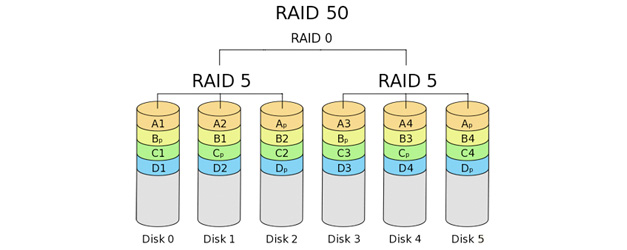
\includegraphics[width=\textwidth,height=200pt]{assets/raid-50.jpg} 
	\caption[Raid 50]{Raid 50. (Source: \cite{raid})}
	\label{fig:raid50}
	\end{figure}

	\item La solution précédente est efficace mais ne peut couvrir la perte des données en cas d'incendie. Si tous les disques durs sont touchés, il sera impossible de restaurer les données. Afin de prévenir ce cas défaillant, un système de backup journalier vers un autre centre hospitalier localisé dans une autre ville peut être mis en place. Ainsi, il sera toujours possible de récupérer les données en cas de gros désastre. Un compromis avec un autre hôpital peut être convenu afin de limiter les coûts. (Chaque hôpital peut conserver un backup de l'autre)
\end{itemize}

\subsubsection{Dosage de médicament encodé de manière erronée}
\justify
\begin{itemize}
	\item Prévoir des séances de formation à l'encodage des données
	\item Permettre plusieurs unités de mesures dans le logiciel. Ainsi, le logiciel peut convertir le dosage dans d'autres unités si nécessaire.
	\item Prévoir des message d'information si le dosage semble trop élevé ou trop faible. (avec pop-up de confirmation)
\end{itemize}

\subsubsection{Mauvaise programmation du système automatisé de gestion du stock}
\justify
\begin{itemize}
	\item Prévoir des séances de formation pour les gestionnaires de stock
	\item Prévoir des aides dans le logiciel afin d'avertir si la programmation est cohérente par rapport à l'existant. (~= détecteur d'anomalie)
\end{itemize}

\subsubsection{Incendie dans la salle des serveurs}
\justify
\begin{itemize}
	\item Voir section \ref{surtension-elec}
	\item Prévoir des détecteurs de fumée.
	\item Prévoir des portes coupe-feu.
	\item Prévoir des extincteurs automatique à gaz neutre. Contrairement aux extincteurs automatiques à eau, le matériel informatique n'est pas abîmé par l'eau. Les gaz extincteurs vont permettre d'étouffer le feu sans abîmer les composants.
\end{itemize}

\subsubsection{Panne de serveur}
\justify
\begin{itemize}
	\item Prévoir un mécanisme de Fail-Over. Les illustrations ci-dessous représentent le scénario d'un mécanisme de failover.
	\begin{figure}[H]
	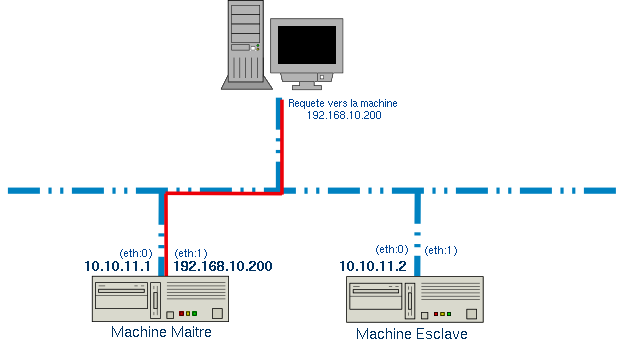
\includegraphics[width=\textwidth,height=200pt]{assets/failover-ok.png} 
	\caption[Failover cas normal]{Système fonctionnel. (Source: \cite{failover})}
	\label{fig:failoverok}
	\end{figure}
	Si la machine maitre tombe en panne. La machine esclave est capable de reprendre la main. Ainsi, le système peut toujours fonctionner en attendant que la première machine soit remplacée.
	\begin{figure}[H]
	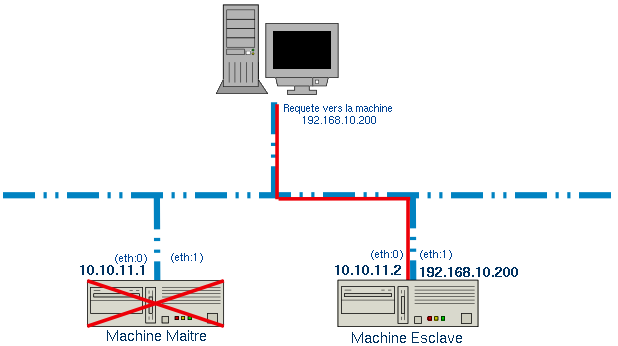
\includegraphics[width=\textwidth,height=200pt]{assets/failover-nok.png} 
	\caption[Failover cas dégradé]{Réatribution des responsabilités à la machine esclave. (Source: \cite{failover})}
	\label{fig:failovernok}
	\end{figure}	
	\item Voir section \ref{dysf-mat}
\end{itemize}

\subsubsection{Infection par un virus informatique}
\justify
\begin{itemize}
	\item Pour les ordinateurs, l'accès à internet n'est pas obligatoire. Le simple accès à la plateforme est nécessaire. Il suffit de ne pas donner un accès à internet à ces machines.
	\item Pour les serveurs, il est nécessaire d'installer au minimum un antivirus.
	\item Pour les serveurs, il est important de désactiver tous les ports inutiles.
	\item Le routeur qui mène à internet possède déjà un firewall. Par contre, la configuration de celui-ci n'est pas à jour. Il faudrait configurer ce routeur afin de bloquer tout le traffic qui n'est pas nécessaire pour l'hôpital.
\end{itemize}

\subsubsection{Récupération de données confidentielles}
\justify
\begin{itemize}
	\item Mettre en place un mécanisme de cryptographie asymétrique afin de sécuriser le transport des données critiques entre l'ordinateur et le serveur applicatif. L'ordinateur va chiffrer les données à envoyer avec clé publique du serveur. De l'autre côté, le serveur va pouvoir déchiffrer le message envoyé par l'ordinateur avec sa clé privée. Il sera le seul à pouvoir lire ce message.
	\begin{figure}[H]
	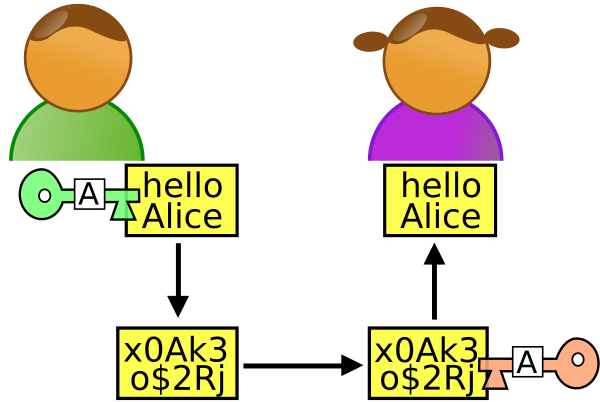
\includegraphics[width=\textwidth,height=200pt]{assets/Asymmetric_cryptography.png} 
	\caption[Mécanisme de cryptographie asymétrique]{Mécanisme de cryptographie asymétrique. (Source: \cite{asymetric-cryptography})}
	\label{fig:cryptoasym}
	\end{figure}
	\item Sécuriser l'accès aux bases de données avec par nom d'utiliseur/mot de passe. Il faut penser à utiliser des utilisateurs spécifiques pour les applications. Ainsi, les droits d'accès peuvent être géré plus facilement. (pas accès à la modification/suppression de schéma, colonnes, etc)
\end{itemize}
	
\subsubsection{Altération des données de connexion}
\hspace{16pt}\textbf{Administrateur système externe:}
\justify
\begin{itemize}
	\item Réduire les droits d'accès. Donner uniquement les accès suffisants.
\end{itemize}


\subsubsection{Suppression des données}
\justify
\hspace{16pt}\textbf{Administrateur système externe:}
\begin{itemize}
	\item Réduire les droits d'accès. Donner uniquement les accès suffisants.
\end{itemize}

\subsubsection{Corruption des données}
\hspace{16pt}\textbf{Erreur matériel:} 
\justify
\begin{itemize}
	\item Si une corruption de données est causée par le disque dur, il est nécessaire d'avoir un mécanisme de récupération de données. Voir section \ref{panne-disque}
\end{itemize}

\subsection{Mesures de sécurité}

\tiny
\begin{longtable}[c]{|
>{\columncolor[HTML]{FCFF2F}}l |c|c|c|c|c|c|c|c|c|c|c|c|l|l|l|c|c|c|c|c|}
\hline
\multicolumn{1}{|c|}{\cellcolor[HTML]{FFCC67}{\color[HTML]{333333} \textbf{\begin{tabular}[c]{@{}c@{}}Mesure\\ de\\ sécurité\end{tabular}}}} & \cellcolor[HTML]{FD6864}\textbf{\begin{tabular}[c]{@{}c@{}}R\\ 1\end{tabular}} & \cellcolor[HTML]{FD6864}\textbf{\begin{tabular}[c]{@{}c@{}}R\\ 2\end{tabular}} & \cellcolor[HTML]{FD6864}\textbf{\begin{tabular}[c]{@{}c@{}}R\\ 3\end{tabular}} & \cellcolor[HTML]{FD6864}\textbf{\begin{tabular}[c]{@{}c@{}}R\\ 4\end{tabular}} & \cellcolor[HTML]{FD6864}\textbf{\begin{tabular}[c]{@{}c@{}}R\\ 5\end{tabular}} & \cellcolor[HTML]{FD6864}\textbf{\begin{tabular}[c]{@{}c@{}}R\\ 6\end{tabular}} & \cellcolor[HTML]{FD6864}\textbf{\begin{tabular}[c]{@{}c@{}}R\\ 7\end{tabular}} & \cellcolor[HTML]{FD6864}{\color[HTML]{333333} \textbf{\begin{tabular}[c]{@{}c@{}}R\\ 8\end{tabular}}} & \cellcolor[HTML]{FD6864}{\color[HTML]{333333} \textbf{\begin{tabular}[c]{@{}c@{}}R\\ 9\end{tabular}}} & \cellcolor[HTML]{FD6864}{\color[HTML]{333333} \textbf{\begin{tabular}[c]{@{}c@{}}R\\ 1\\ 0\end{tabular}}} & \cellcolor[HTML]{FD6864}{\color[HTML]{333333} \textbf{\begin{tabular}[c]{@{}c@{}}R\\ 1\\ 1\end{tabular}}} & \cellcolor[HTML]{FD6864}{\color[HTML]{333333} \textbf{\begin{tabular}[c]{@{}c@{}}R\\ 1\\ 2\end{tabular}}} & \multicolumn{1}{c|}{\cellcolor[HTML]{FD6864}\textbf{\begin{tabular}[c]{@{}c@{}}R\\ 1\\ 3\end{tabular}}} & \multicolumn{1}{c|}{\cellcolor[HTML]{FD6864}\textbf{\begin{tabular}[c]{@{}c@{}}R\\ 1\\ 4\end{tabular}}} & \multicolumn{1}{c|}{\cellcolor[HTML]{FD6864}\textbf{\begin{tabular}[c]{@{}c@{}}R\\ 1\\ 5\end{tabular}}} & \cellcolor[HTML]{C0C0C0}\textbf{\begin{tabular}[c]{@{}c@{}}Bien\\ sup-\\ port\\ sur \\ lequel\\ elle \\ repose\end{tabular}} & \cellcolor[HTML]{32CB00}\textbf{\begin{tabular}[c]{@{}c@{}}Thème \\ ISO\\ 27002\end{tabular}} & \cellcolor[HTML]{34CDF9}\textbf{\begin{tabular}[c]{@{}c@{}}Pré-\\ vention\end{tabular}} & \cellcolor[HTML]{34CDF9}\textbf{\begin{tabular}[c]{@{}c@{}}Pro-\\ tection\end{tabular}} & \cellcolor[HTML]{34CDF9}\textbf{\begin{tabular}[c]{@{}c@{}}Récu-\\ pération\end{tabular}} \\ \hline
\endhead
%
\begin{tabular}[c]{@{}l@{}}Prévoir\\ plusieurs\\ groupes\\ élèctrogènes\end{tabular} & X &  &  &  &  &  &  &  & X &  &  &  &  &  &  & \begin{tabular}[c]{@{}c@{}}SYS\\ Reseau\\ interne\end{tabular} & \begin{tabular}[c]{@{}c@{}}11.\\ Sécurité\\ physique\\ et\\  environ-\\ nementale\end{tabular} &  &  & X \\ \hline
\begin{tabular}[c]{@{}l@{}}Prévoir\\ des batteries\\ au lithium-\\ ion\end{tabular} & X &  &  &  &  &  &  &  & X &  &  &  &  &  &  & \begin{tabular}[c]{@{}c@{}}SYS\\ Reseau\\ interne\end{tabular} & \begin{tabular}[c]{@{}c@{}}11.\\ Sécurité\\ physique\\ et\\  environ-\\ nementale\end{tabular} &  &  & X \\ \hline
\begin{tabular}[c]{@{}l@{}}Prévoir des\\ bateries à\\ l'hydrogène\end{tabular} & X &  &  &  &  &  &  &  & X &  &  &  &  &  &  & \begin{tabular}[c]{@{}c@{}}SYS\\ Reseau\\ interne\end{tabular} & \begin{tabular}[c]{@{}c@{}}11.\\ Sécurité\\ physique\\ et\\  environ-\\ nementale\end{tabular} & \multicolumn{1}{l|}{} &  & X \\ \hline
\begin{tabular}[c]{@{}l@{}}Prévoir des\\ disjoncteurs\end{tabular} & X & X &  &  &  &  &  &  & X &  &  &  &  &  &  & \begin{tabular}[c]{@{}c@{}}SYS\\ Reseau\\ interne\end{tabular} & \begin{tabular}[c]{@{}c@{}}11.\\ Sécurité\\ physique\\ et\\  environ-\\ nementale\end{tabular} & \multicolumn{1}{l|}{} & X & \multicolumn{1}{l|}{} \\ \hline
\begin{tabular}[c]{@{}l@{}}Installer des\\ parafoudres\\ aux points\\ d'entrée des\\ câbles\end{tabular} & X &  &  &  &  &  &  &  &  &  &  &  &  &  &  & \begin{tabular}[c]{@{}c@{}}SYS\\ Reseau\\ interne\end{tabular} & \begin{tabular}[c]{@{}c@{}}11.\\ Sécurité\\ physique\\ et\\  environ-\\ nementale\end{tabular} & \multicolumn{1}{l|}{} & X & \multicolumn{1}{l|}{} \\ \hline
\begin{tabular}[c]{@{}l@{}}Ajouter des\\ étiquettes\\ sur les cables\end{tabular} & X &  &  &  &  &  &  &  &  &  &  &  &  &  &  & \begin{tabular}[c]{@{}c@{}}SYS\\ Réseau\\ interne\end{tabular} & \begin{tabular}[c]{@{}c@{}}11.\\ Sécurité\\ physique\\ et\\  environ-\\ nementale\end{tabular} & X &  &  \\ \hline
\begin{tabular}[c]{@{}l@{}}Prévoir\\ deux ali-\\ mentations\end{tabular} & X &  &  &  &  &  &  &  &  & X &  &  &  &  &  & \begin{tabular}[c]{@{}c@{}}SYS\\ Réseau\\ interne\end{tabular} & \begin{tabular}[c]{@{}c@{}}11.\\ Sécurité\\ physique\\ et\\  environ-\\ nementale\end{tabular} &  & X & X \\ \hline
\begin{tabular}[c]{@{}l@{}}Prévoir des\\ pièces de\\ rechanges\end{tabular} &  & X & X &  &  & X &  &  &  & X &  &  &  &  &  & \begin{tabular}[c]{@{}c@{}}SYS\\ Réseau\\ interne\end{tabular} & \begin{tabular}[c]{@{}c@{}}11.\\ Sécurité\\ physique\\ et\\  environ-\\ nementale\end{tabular} &  &  & X \\ \hline
\begin{tabular}[c]{@{}l@{}}Service\\ de dépan-\\ nage 24h/24\end{tabular} &  & X & X &  &  & X &  &  &  & X &  &  &  &  &  & \begin{tabular}[c]{@{}c@{}}SYS\\ Réseau\\ interne\end{tabular} & \begin{tabular}[c]{@{}c@{}}14.\\ Acquisition,\\ dévelop-\\ pement et \\ maintenan-\\ ce des sys-\\ tèmes d’in-\\ formation\end{tabular} &  &  & X \\ \hline
\begin{tabular}[c]{@{}l@{}}Système d'\\ authentifi-\\ cation de\\ secours\end{tabular} & X &  & X &  &  &  &  &  &  &  &  &  &  &  &  & \begin{tabular}[c]{@{}c@{}}MAT\\ Serveur\end{tabular} & \begin{tabular}[c]{@{}c@{}}9.\\ Contrôle\\ d'accès\end{tabular} &  &  & X \\ \hline
\begin{tabular}[c]{@{}l@{}}Ajouter\\ des logs\end{tabular} &  &  & X &  &  &  &  &  &  & X &  &  &  &  &  & \begin{tabular}[c]{@{}c@{}}MAT\\ Serveur\end{tabular} & \begin{tabular}[c]{@{}c@{}}12.\\ Sécurité\\ liée à l’\\ exploitation\end{tabular} & X &  &  \\ \hline
\begin{tabular}[c]{@{}l@{}}Ajouter des\\ exceptions\end{tabular} &  &  & X &  &  &  &  &  &  & X &  &  &  &  &  & \begin{tabular}[c]{@{}c@{}}MAT\\ Serveur\end{tabular} & \begin{tabular}[c]{@{}c@{}}12.\\ Sécurité\\ liée à l’\\ exploitation\end{tabular} & X &  &  \\ \hline
\begin{tabular}[c]{@{}l@{}}Prévoir des\\ avertis-\\ sement dans\\ l'interface\\ graphique\end{tabular} & \textit{} & X & X &  & \textit{} & X & X & X &  & X &  &  &  &  &  & \begin{tabular}[c]{@{}c@{}}MAT\\ Serveur\end{tabular} & \begin{tabular}[c]{@{}c@{}}12.\\ Sécurité\\ liée à l’\\ exploitation\end{tabular} & X &  &  \\ \hline
\begin{tabular}[c]{@{}l@{}}Bouton\\ d'aide vers\\ des techni-\\ ciens en cas\\ de problème\end{tabular} &  & X & X &  &  & X & X &  &  & X &  &  &  &  &  & \begin{tabular}[c]{@{}c@{}}MAT\\ Serveur\end{tabular} & \begin{tabular}[c]{@{}c@{}}14.\\ Acquisition,\\ dévelop-\\ pement et \\ maintenan-\\ ce des sys-\\ tèmes d’in-\\ formation\end{tabular} & X &  &  \\ \hline
\begin{tabular}[c]{@{}l@{}}Fiche de\\ prévention\end{tabular} &  &  &  & X &  &  &  &  &  &  &  &  &  &  &  & \begin{tabular}[c]{@{}c@{}}MAT\\ Ordinateur\end{tabular} & \begin{tabular}[c]{@{}c@{}}7.\\ La sécurité\\ des ressources\\ humaines\end{tabular} & X & \multicolumn{1}{l|}{} & \multicolumn{1}{l|}{} \\ \hline
\begin{tabular}[c]{@{}l@{}}Authentifi-\\ cation à \\ plusieurs \\ facteurs\end{tabular} &  &  &  &  & X &  &  &  &  &  &  &  &  &  &  & \begin{tabular}[c]{@{}c@{}}MAT\\ Ordinateur\end{tabular} & \begin{tabular}[c]{@{}c@{}}9.\\ Contrôle d’\\ accès\end{tabular} & \multicolumn{1}{l|}{} & X & X \\ \hline
\begin{tabular}[c]{@{}l@{}}Désactiva-\\ tion de badge\end{tabular} &  &  &  &  & X &  &  &  &  &  &  &  &  &  &  & \begin{tabular}[c]{@{}c@{}}MAT\\ Serveur\end{tabular} & \begin{tabular}[c]{@{}c@{}}8.\\ Gestion\\ des actifs\end{tabular} & \multicolumn{1}{l|}{} & X & \multicolumn{1}{l|}{} \\ \hline
\begin{tabular}[c]{@{}l@{}}Système d'\\ ap-probation\end{tabular} &  &  &  &  &  &  &  & X &  &  &  &  &  &  &  & \begin{tabular}[c]{@{}c@{}}MAT\\ Serveur\end{tabular} & \begin{tabular}[c]{@{}c@{}}12.\\ Système\\ d'approbation\end{tabular} & X & X & \multicolumn{1}{l|}{} \\ \hline
RAID 50 &  &  &  &  &  & X &  &  &  &  &  &  &  &  &  & \begin{tabular}[c]{@{}c@{}}MAT\\ Disques\\ durs\end{tabular} & \begin{tabular}[c]{@{}c@{}}12.\\ Sécurité\\ liée à l’\\ exploitation\end{tabular} & \multicolumn{1}{l|}{} & X & X \\ \hline
\begin{tabular}[c]{@{}l@{}}Backup\\ multi-site\end{tabular} &  &  &  &  &  & X &  &  &  &  &  &  &  & \multicolumn{1}{c|}{X} & \multicolumn{1}{c|}{X} & \begin{tabular}[c]{@{}c@{}}MAT\\ Disques\\ durs\end{tabular} & \begin{tabular}[c]{@{}c@{}}12.\\ Sécurité\\ liée à l’\\ exploitation\end{tabular} & \multicolumn{1}{l|}{} & X & X \\ \hline
\begin{tabular}[c]{@{}l@{}}Séance de\\ formation\end{tabular} &  &  &  &  &  &  & X & X &  &  &  &  &  &  &  & \begin{tabular}[c]{@{}c@{}}ORG\\ Organisa-\\ tion de l'\\ hôpital\end{tabular} & \begin{tabular}[c]{@{}c@{}}7.\\ La sécurité\\ des res-\\ sources\\ humaines\end{tabular} & X & \multicolumn{1}{l|}{} & \multicolumn{1}{l|}{} \\ \hline
\begin{tabular}[c]{@{}l@{}}Pop-up\\ d'aide dans\\ l'interface\end{tabular} &  &  & X &  &  &  & X & X &  &  &  &  &  &  &  & \begin{tabular}[c]{@{}c@{}}MAT\\ Serveur\end{tabular} & \begin{tabular}[c]{@{}c@{}}12.\\ Sécurité\\ liée à l’\\ exploitation\end{tabular} & X & \multicolumn{1}{l|}{} & \multicolumn{1}{l|}{} \\ \hline
\begin{tabular}[c]{@{}l@{}}Detecteur\\ de fumée\end{tabular} &  &  &  &  &  &  &  &  & X &  &  &  &  &  &  & \begin{tabular}[c]{@{}c@{}}LOC\\ Locaux\end{tabular} & \begin{tabular}[c]{@{}c@{}}11.\\ Sécurité\\ physique\\ et\\ environ-\\ nementale\end{tabular} & X & \multicolumn{1}{l|}{} & \multicolumn{1}{l|}{} \\ \hline
\begin{tabular}[c]{@{}l@{}}Porte\\ coupe-feu\end{tabular} &  &  &  &  &  &  &  &  & X &  &  &  &  &  &  & \begin{tabular}[c]{@{}c@{}}LOC\\ Locaux\end{tabular} & \begin{tabular}[c]{@{}c@{}}11.\\ Sécurité\\ physique\\ et\\ environ-\\ nementale\end{tabular} & \multicolumn{1}{l|}{} & X & X \\ \hline
\begin{tabular}[c]{@{}l@{}}Extincteur\\ automatique\\ à gaz\end{tabular} &  &  &  &  &  &  &  &  & X &  &  &  &  &  &  & \begin{tabular}[c]{@{}c@{}}LOC\\ Locaux\end{tabular} & \begin{tabular}[c]{@{}c@{}}11.\\ Sécurité\\ physique\\ et\\ environ-\\ nementale\end{tabular} & \multicolumn{1}{l|}{} & X & X \\ \hline
\begin{tabular}[c]{@{}l@{}}Mécanisme\\ de Fail-Over\end{tabular} & X & X &  &  &  &  &  &  &  & X &  &  &  &  &  & \begin{tabular}[c]{@{}c@{}}MAT\\ Serveur\end{tabular} & \begin{tabular}[c]{@{}c@{}}12.\\ Sécurité\\ liée à l’\\ exploitation\end{tabular} & \multicolumn{1}{l|}{} & X & X \\ \hline
\begin{tabular}[c]{@{}l@{}}Retirer la\\ connexion\\ à internet\end{tabular} &  &  &  &  &  &  &  &  &  &  & X &  &  &  &  & \begin{tabular}[c]{@{}c@{}}MAT\\ Ordinateur\end{tabular} & \begin{tabular}[c]{@{}c@{}}12.\\ Sécurité\\ liée à l’\\ exploitation\end{tabular} & X & \multicolumn{1}{l|}{} & \multicolumn{1}{l|}{} \\ \hline
\begin{tabular}[c]{@{}l@{}}Installer\\ un anti-virus\end{tabular} &  &  &  &  &  &  &  &  &  &  & X &  &  &  &  & \begin{tabular}[c]{@{}c@{}}MAT\\ Ordinateur\\ Serveur\end{tabular} & \begin{tabular}[c]{@{}c@{}}12.\\ Sécurité\\ liée à l’\\ exploitation\end{tabular} & X & X & \multicolumn{1}{l|}{} \\ \hline
\begin{tabular}[c]{@{}l@{}}Désactiver\\ les ports\\ inutiles\end{tabular} &  &  &  &  &  &  &  &  &  &  & X &  &  &  &  & \begin{tabular}[c]{@{}c@{}}SYS\\ Réseau\\ interne\end{tabular} & \begin{tabular}[c]{@{}c@{}}12.\\ Sécurité\\ liée à l’\\ exploitation\end{tabular} & X & X & \multicolumn{1}{l|}{} \\ \hline
\begin{tabular}[c]{@{}l@{}}Configurer\\ le firewall\\ afin de \\ bloquer les\\ sites non-\\ nécessaires\end{tabular} &  &  &  &  &  &  &  &  &  &  & X &  &  &  &  & \begin{tabular}[c]{@{}c@{}}SYS\\ Réseau\\ interne\end{tabular} & \begin{tabular}[c]{@{}c@{}}12.\\ Sécurité\\ liée à l’\\ exploitation\end{tabular} & X & X &  \\ \hline
\begin{tabular}[c]{@{}l@{}}Mécanisme\\ de crypto-\\ graphie \\ asymétrique\end{tabular} &  &  &  &  &  &  &  &  &  &  &  & X &  &  &  & \begin{tabular}[c]{@{}c@{}}SYS\\ Réseau\\ interne\end{tabular} & \begin{tabular}[c]{@{}c@{}}10.\\ Cryptographie\end{tabular} &  & X &  \\ \hline
\begin{tabular}[c]{@{}l@{}}Authentifi-\\ cation\\ user/password\end{tabular} &  &  &  &  &  &  &  &  &  &  &  &  & \multicolumn{1}{c|}{X} & \multicolumn{1}{c|}{X} & \multicolumn{1}{c|}{} & \begin{tabular}[c]{@{}c@{}}SYS\\ Réseau\\ interne\end{tabular} & \begin{tabular}[c]{@{}c@{}}9.\\ Contrôle d’\\ accès\end{tabular} &  & X &  \\ \hline
\begin{tabular}[c]{@{}l@{}}Réduire les\\ droits d'accès\end{tabular} &  &  &  &  &  &  &  &  &  &  &  &  & \multicolumn{1}{c|}{X} & \multicolumn{1}{c|}{X} & \multicolumn{1}{c|}{X} & \begin{tabular}[c]{@{}c@{}}MAT\\ Serveur\\ AD\end{tabular} & \begin{tabular}[c]{@{}c@{}}9.\\ Contrôle d’\\ accès\end{tabular} & X & X &  \\ \hline
\caption{Tableau des mesures de sécurité}
\label{tab:mesure-de-securite}\\
\end{longtable}

\newpage

%---------------------------------------List of Figures----------------------------------------

\section*{Table des figures}
\makeatletter
\@starttoc{lof}% Print List of Figures
\makeatother
\addcontentsline{toc}{section}{\protect\numberline{}Table des figures}%
%---------------------------------------List of Tables----------------------------------------
\section*{Liste des tableaux}
\makeatletter
\@starttoc{lot}% Print List of Tables
\makeatother
\addcontentsline{toc}{section}{\protect\numberline{}Liste des tableaux}%
%---------------------------------------References----------------------------------------

\nocite{*}
\section*{Bibliographie}

\printbibliography[heading=none]

\addcontentsline{toc}{section}{\protect\numberline{}Bibliographie}%

%----------------------------------------------------------------------------------------
%----------------------------------------THE END-----------------------------------------
%----------------------------------------------------------------------------------------

\end{document}
